\problemname{Planet Slope}

In a not too distant future, scientists have discovered not only \emph{one} previously unknown planet here in our own solar system (see the problem Planet X) but now \emph{yet another one}, called planet Y.

The scientists are interested in what the topography on Planet Y looks like, and have managed to measure this with great accuracy. We represent the surface as an $N \times M$ grid, where each cell has a measured height between $0$ and $9$.

To the delight of many, it turns out that planet Y has a perfect climate for skiing (as you surely understand, there is no longer any snow on Earth at this point). Write a program that computes the longest ski slope that can be built on planet Y.

\begin{figure}[h]
  \centering
      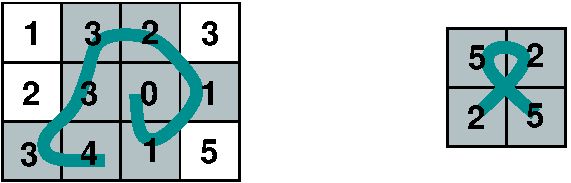
\includegraphics[width=0.7\textwidth]{planetbackefig2}
      \caption{On the left the first sample is shown and on the right the second sample. The thick line shows the path of the ski slope and the shaded cells are the cells that are part of the ski slope.}
\end{figure}

The requirement for a ski slope is that it must be a connected sequence of cells where each pair of cells is adjacent either via a shared side or a shared corner (see the figures above), and where each cell in the sequence has a height no greater than the previous one. It is thus allowed in principle for all cells in the ski slope to have the same height. The same cell may not be used more than once, but the ski slope could still cross itself through a corner as in the second sample below.

\section*{Input}
The first line contains two integers $1 \le N,M \le 7$,
the number of rows and columns in the grid.
Then follow $N$ lines with $M$ characters each.
The $j$-th character on line $i$ is a digit between
$0$ and $9$ corresponding to the height of the cell. There are never more than $7$ cells in the grid with the same height.

\section*{Output}
The program should print an integer: the largest number of cells that can be part of a valid ski slope.

\section*{Scoring}
Your solution will be tested on a set of test groups.
To earn points for a group, you must pass all test cases in that group.

\noindent
\begin{tabular}{| l | l | l |}
  \hline
  \textbf{Group} & \textbf{Points} & \textbf{Constraints} \\ \hline
  $1$    & $20$        &  $1 \leq M, N \leq 3$\\ \hline
  $2$    & $20$        &  No adjacent cells have the same height. \\ \hline
  $3$    & $20$        &  Each cell is adjacent to at most two cells with the same height as itself. \\ \hline
  $4$    & $40$        &  No additional constraints. \\ \hline
\end{tabular}
